% !TeX root = Body.tex
\chapter{Numerical Simulations}\label{chap:NumSim}

In this chapter, we present the way of calculating the frictional force as a non-equilibrium physical quantity. This method for lattice spin systems was first introduced by Kadau \textit{et al}.\ \cite{Kadau2008} and has widely used in related works until now \cite{Hucht2009b,Magiera2011,Igloi2011,Hucht2012a,Angst2012,Li2016b}. We also explain, in particular, the convergence to the non-equilibrium steady state by our Monte Carlo simulation method.

\section{Setup of the Model}\label{sec:SetupModel}
Sliding friction is a form of energy dissipation on the surface between a moving object and its substrate. The dissipated energy is originated in the kinetic energy of the moving object. We here consider a constantly moving case in which an external force maintains the motion of the object with endless supply of its kinetic energy. This view leads to its \textit{non-equilibrium stationary state} (see Fig.~\ref{fig:schemNESS}). We will show in Fig.~\ref{fig:timeseries} below our simulation data of the energy changes.
\begin{figure}[htbp]
	\centering
	\subcaptionbox{\label{subcap:schemNESS1}}[0.32\linewidth]{\includegraphics[height=0.15\linewidth]{schemNESS1.png}}
	\subcaptionbox{\label{subcap:schemNESS2}}[0.32\linewidth]{\includegraphics[height=0.15\linewidth]{schemNESS2.png}}
	\subcaptionbox{\label{subcap:schemNESS3}}[0.32\linewidth]{\includegraphics[height=0.15\linewidth]{schemNESS3.png}}
	
	\caption{Schematic picture of a moving object and a substrate. If the whole system is in the equilibrium state (\subref{subcap:schemNESS1}), the motion of the upper object makes a change of the boundary energy, which has a positive value in the ensemble average (\subref{subcap:schemNESS2}). Interacting with the surrounding environment, the system tries to relax to the equilibrium state again (\subref{subcap:schemNESS3}). The perpetual motion by an external force, however, prevents the system from going back to the equilibrium state; instead the system goes to the non-equilibrium stationary state.}
	\label{fig:schemNESS}
\end{figure}

When the system is in a non-equilibrium stationary state, it is often easy to calculate \textit{energy currents} such as the frictional heat, its power and so on. Applying the view to our case in which two square lattices of the Ising model slide against each other, we can formulate the problem as follows; see Fig.~\ref{fig:CutIsing}.
\begin{enumerate}
	\item We prepare a square lattice of the Ising model of size $L_{x}\times L_{z}$ and impose periodic boundary conditions in the transverse ($x$) direction, whereas we set the open boundary conditions in the longitudinal ($z$) direction for the moment. We first set the system in the equilibrium state of a temperature $T$.
	\item We cut the system along the $x$-direction into two parts, maintaining interactions on the cut.
	\item We slide two parts along the cut plane with relative velocity $v$. In other words, we shift the upper half by a lattice constant every $1/v$ unit time. 
\end{enumerate}

\begin{figure}[htbp]
	\centering
	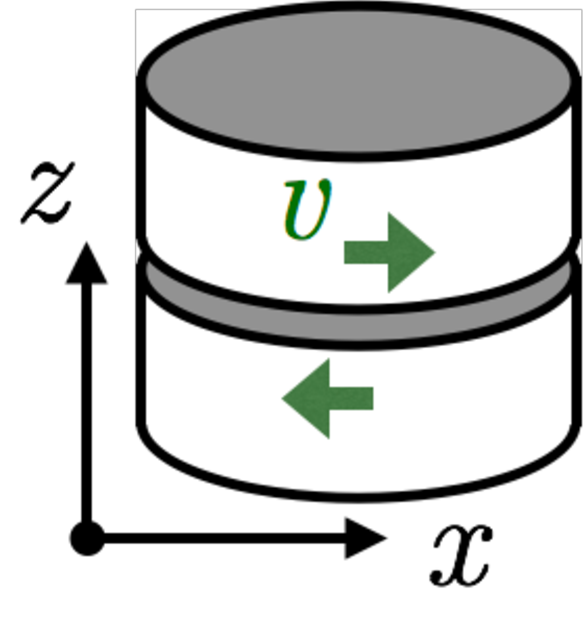
\includegraphics[width=0.25\linewidth]{CutIsing.pdf}
	\caption{Two cylinders of the Ising model sliding with the velocity $v$.}
	\label{fig:CutIsing}
\end{figure}
The Hamiltonian of the system is given by
\begin{align}
&H=H_{\rm upper} + H_{\rm lower} + H_{\rm slip}(t),
\end{align}
where
\begin{align}
&H_{\rm upper}:=-J\sum_{\langle i,j\rangle\in\mathrm{upper}}\sigma_{i}\sigma_{j}\label{ham:upper}, \\
&H_{\rm lower}:=-J\sum_{\langle i,j\rangle\in\mathrm{lower}}\sigma_{i}\sigma_{j}\label{ham:lower}, \\
&H_{\rm slip}(t):=-J\sum_{\langle i,j(t)\rangle\in\mathrm{slip}}\sigma_{i}\sigma_{j(t)}\label{ham:slip}
\end{align}
with the subscripts upper, lower and slip representing the set of neighboring spin pairs on the upper half, the lower half and the slip plane, respectively. In $H_{\rm slip}(t)$, the $i$th spin on the boundary above the cut changes the opponent of the interaction on the boundary below the cut as indicated by $j(t)$ when the upper lattice shifts against the lower one. We alternate the shift operations and the Monte Carlo spin flips in our simulation. We will give the details of the simulation schedule below in Sec.~\ref{subsec:SlipPlaneWithV}.

Shift operations on the upper lattice lead the system to repeated \textit{pumping} and \textit{dissipation} processes as follows:
\begin{enumerate}
	\item \textbf{Shift}: A shift operation excites the energy on the slip plane by the amount $\langle H_{\rm slip}(t')-H_{\rm slip}(t)\rangle_{\rm st}$, where the letter $t'$ denotes the time just after the shift operation at time $t$.
	\item \textbf{Relax 1}: The excited energy on the slip plane $\langle H_{\rm slip}(t')-H_{\rm slip}(t)\rangle_{\rm st}$ dissipates to the entire system.
	\item \textbf{Relax 2}: The excited entire system relaxes towards the equilibrium.
\end{enumerate}
Our model always reaches a non-equilibrium stationary states in the long-time limit $t\to\infty$, which depends on the temperature $T$ and the sliding velocity $v$; see Sec.~\ref{subsec:convproof} for the proof. We define the stationary-state average $\langle A\rangle_{\rm st}:=\sum_{i}A_{i}p^{(\rm st)}_{i}$ for an arbitrary observable $A$, where $\{A_{i}\}$ are observed values of $A$ and $p^{(\rm st)}_{i}$ denotes the stationary-state probability distribution, which is different from the equilibrium (canonical) probability distribution $p^{(\rm eq)}_{i}\propto\exp\left[-E_{i}/(k_{\rm B} T)\right]$.

\section{Non-equilibrium Monte Carlo Simulation}
The dissipation process towards the heat bath occurs via a spin flip. This fundamental processes do not only describe the equilibrium state but also the non-equilibrium stationary state at a fixed temperature parameter $T$~\cite{Glauber1963}. Using the Monte Carlo method, we simulate this process.

\subsection{Introduction of the Time Scale to Ising Models}
In order to calculate dynamical observables such as the frictional power \eqref{def:Pump} and its dissipation rate \eqref{def:Diss}, we have to define \textit{a unit time} for the simulation of the finite-size system. 

For the equilibrium Monte Carlo simulation, the most naive approach for the equilibrium state is the single-spin-flip algorithm, where we perform the sequence of a random selection of a spin and its flip with a temperature-dependent probability $p(T)$. We use the probability that satisfies the \textit{detailed balance condition}, which certainly leads the system towards the true equilibrium state with enough repetition of the sequence. For example, we often use the Metropolis probability $p_{\rm M}(T):=\min\{1,\exp\left[-\Delta E/(k_{\rm B}T)\right]\}$ as the probability $p(T)$, where $\Delta E$ is the energy difference due to the flip. We often call a \textit{Monte Carlo step} a single process of the algorithm, and define a \textit{Monte Carlo sweep} by $N$ Monte Carlo steps, where $N$ is the number of spins.

Which should we use as a unit time, a Monte Carlo step or a Monte Carlo sweep? Its answer can be found in the following manner. We usually assume that a statistical mechanical system is coupled to a heat bath by every local degree of freedom. The temperature of the system is kept constant by the heat bath, and the system exchanges its energy with the heat bath through local degrees of freedom. It is most symmetric to assume that the equilibrium relaxation of a macroscopic system takes place in the same time scale if the volume of the system is doubled. Thus the number of times of the energy exchanges is proportional to the total number of degrees of freedom of the system. This justifies to define a unit time by a Monte Carlo sweep; the relaxation time would be proportional to the total number of degrees of freedom if we used the Monte Carlo steps for a unit time.

\subsection{Slip Plane with the Velocity $v$}\label{subsec:SlipPlaneWithV}
Using the introduced time scale, we can also introduce the sliding velocity $v$ of the system with $N$ spins, where $N=L_{x}\times L_{z}$. Corresponding to the setup in Sec.~\ref{sec:SetupModel}, we perform an extended single-spin-flip algorithm with the following unit Monte Carlo time:
\begin{enumerate}
	\item \textbf{Shift}: We shift the upper half of the lattice by a lattice constant.
	\item \textbf{Flip}: We perform ordinary single flips for $(N/v)$ times, which is the $(1/v)$ fraction of a Monte Carlo sweep.
	\item We repeat the processes 1 and 2 for $v$ times.
\end{enumerate}
In the extended algorithm, the upper half slides with the velocity $v$ in a unit time at regular intervals. The frictional power $P(t)$ and the dissipation rate $D(t)$ are measured in Monte Carlo simulations as the energy differences for a unit time due to the shift and the flip operation, respectively (see Section~\ref{sec:defquan} for definitions of the frictional power $P(t)$ and the dissipation rate $D(t)$).

Magnetic frictions in the Ising model are described by the following elementary process. Suppose that the system is in an equilibrium state with a snapshot as in Fig.~\ref{fig:snapshots}(\subref{subcap:snapshot1}). A sliding operation stretches the domain wall across the sliding boundary as in Fig.~\ref{fig:snapshots}(\subref{subcap:snapshot2}). The stretched domain wall tends to shrink by thermal fluctuations as in Fig.~\ref{fig:snapshots}(\subref{subcap:snapshot3}). The energy of the system jumps at the stretching process and decays at the shrinking process. The sums of these energy changes for a Monte Carlo sweep are equal to our observed quantities $P(t)$ and $D(t)$, respectively.

\begin{figure}[htbp]
	\centering
	\subcaptionbox{\label{subcap:snapshot1}}[0.32\linewidth]{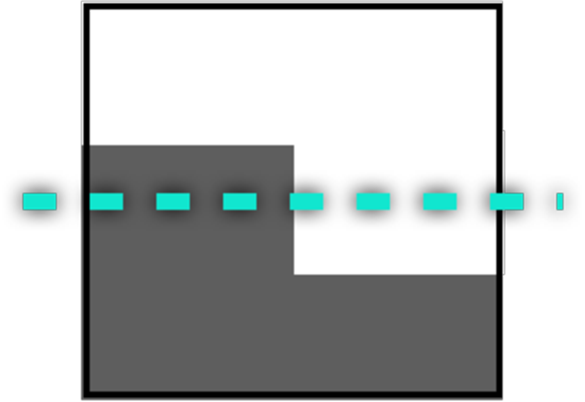
\includegraphics[width=0.25\linewidth]{Snapshot1.pdf}}
	\subcaptionbox{\label{subcap:snapshot2}}[0.32\linewidth]{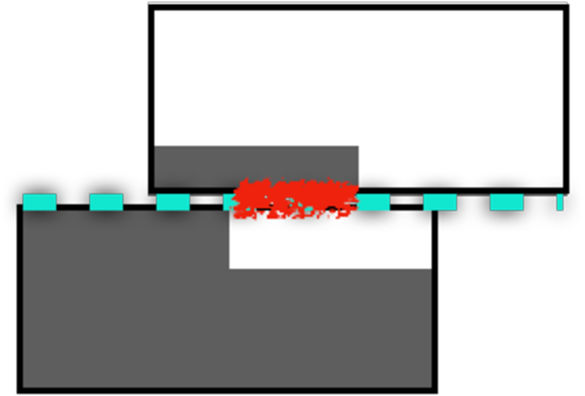
\includegraphics[width=0.25\linewidth]{Snapshot2.pdf}}
	\subcaptionbox{\label{subcap:snapshot3}}[0.32\linewidth]{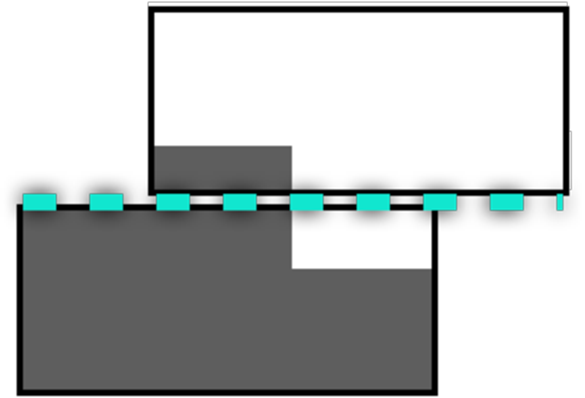
\includegraphics[width=0.25\linewidth]{Snapshot3.pdf}}
	
	\caption{A schematic picture of magnetic frictions in an elementary process.}
	\label{fig:snapshots}
\end{figure}

We show an example of the time series of the bulk energy (see Fig.~\ref{fig:timeseries}). We thermalized the system of size $20\times 20$ for $40{,}000$ MC steps and equilibrated it at the temperature $T=2.50$. We then make the system slide with the constant velocity $v=1$ from the time $t=40{,}001$ MC step for $40{,}000$ MC steps until the time $t=80{,}000$ MC step. The energy takes the value of the equilibrium state just after the start point of sliding (see Fig.~\ref{fig:timeseries}(\subref{subcap:timeseries_ns})). After a sufficient length of the time, however, the average value of the energy converges to a new value of the non-equilibrium stationary state (see Fig.~\ref{fig:timeseries}(\subref{subcap:timeseries_s})). For each $400$ MC steps, which corresponds to a MC sweep, a sliding operation makes the energy \textit{jump} and the relaxation process by spin flips make it \textit{decay}. The sum of contributions to the energy by jump and decay processes for a MC sweep are equal to the value of $P(t)$ and $D(t)$, respectively. Both the frictional power $P(t)$ and the dissipation rate $D(t)$ have the same absolute value in the long-time limit.

\begin{figure}[htbp]
	\centering
	\subcaptionbox{\label{subcap:timeseries_ns}}[0.48\linewidth]{\includegraphics[width=0.45\linewidth]{../../NumCalc/ClassicalSpinMC_tmp/1pass_nonstationary.eps}}
	\subcaptionbox{\label{subcap:timeseries_s}}[0.48\linewidth]{\includegraphics[width=0.45\linewidth]{../../NumCalc/ClassicalSpinMC_tmp/1pass_stationary.eps}}
	
	\caption{Time series of the energy of the whole system in regimes of non-equilibrium relaxation from the equilibrium state (\subref{subcap:timeseries_ns}) and in the non-equilibrium stationary state (\subref{subcap:timeseries_s}).}
	\label{fig:timeseries}
\end{figure}
A comment on our algorithm is in order. The shift operation and spin flips occur in one Monte Carlo sweep but separately, which may or may not reproduce the real situation of relaxation while sliding. A possible alternative is to introduce a distance-dependent exchange interaction between the spins above and below the cut and change the interaction continuously in time. Here we choose to stick to our algorithm for simplicity.
%Note that our simulations capture only the changes of the energy at each MC sweep, in which every sliding process is performed \textit{in an instant}. Conversely, such states are completely neglected that a spin in the lower boundary is located just lower the middle point of two spins in the upper boundary.  To simulate such processes in detail, we have to discuss, for example, the dependence of the interaction between two spins on the distance, which we implement to Monte Carlo simulations.

\subsection{Convergence to the Non-equilibrium Stationary State}\label{subsec:convproof}

The convergence to a unique non-equilibrium stationary state is ensured in the following way. The above algorithm is represented by the following matrix for a Monte Carlo sweep:
\begin{align}
\hat{T}(\beta,v):=\left[\left(\hat{M}(\beta)\right)^{N/v}\hat{S}\right]^{v},
\end{align}
where $v\in\{\text{Divisors of }N\}$. The matrix $\hat{M}(\beta)$ and $\hat{S}$ express a Monte Carlo step at a temperature $T$ and sliding of the upper half by a lattice constant, respectively, for the model of size $N=L_{x}\times L_{z}$. The matrix $\hat{T}(\beta,v)$ describes the time evolution for a Monte Carlo sweep, because the matrix have the $N$th power of $\hat{M}(\beta)$. The matrices $\hat{M}(\beta)$ and $\hat{S}$ belong to the class called the \textit{stochastic matrix}, which is defined by the following properties:
\begin{itemize}
	\item Each element is greater than or equal to zero;
	\item Each row-wise total sum of elements is normalized to unity.
\end{itemize}
The product of two stochastic matrices is also a stochastic matrix. Indeed if we have two $\Omega$-dimensional stochastic matrices $\hat{A}$ and $\hat{B}$, we have
\begin{align}
\sum_{i=1}^{\Omega}(\hat{A}\hat{B})_{ij} = \sum_{i=1}^{\Omega}\sum_{k=1}^{\Omega}A_{ik}B_{kj} = \sum_{k=1}^{\Omega}\left(\sum_{i=1}^{\Omega}A_{ik}\right)B_{kj} = \sum_{k=1}^{\Omega}B_{kj} = 1 \quad\text{for $1\leq j\leq \Omega$},
\end{align}
and therefore the matrix $\left(\hat{M}(\beta)\right)^{N/v}\hat{S}$ is also a stochastic matrix. Any stochastic matrix has at least the eigenvalue $1$ (see App.~\ref{chap:ProofEx}), and therefore the matrix $\left(\hat{M}(\beta)\right)^{N/v}\hat{S}$ also has the eigenvalue $1$.

We now use the concept of \textit{strong connectivity} of stochastic matrices, which ensures that the the eigenvalue $1$ is the only eigenvalue of absolute value $1$ and the moduli of all other eigenvalues are less than $1$. If a stochastic matrix $\hat{A}$ satisfies the condition that any element of the power $\left(\hat{A}\right)^{N_{0}}$ is positive for an integer $N_{0}$, we call the matrix $\hat{A}$ strongly connected. Namely, we can say that if the matrix $\hat{T}(\beta,v)$ is strongly connected the corresponding simulation always converges to the non-equilibrium stationary state.

%We prove that this algorithm leads the system of any size to a non-equilibrium stationary state which depends on the temperature $T$ and the velocity $v$. The above algorithm is represented by the following matrix for a Monte Carlo sweep:
%\begin{align}
%\hat{T}(\beta,v):=\left[\left(\hat{M}(\beta)\right)^{N/v}\hat{S}\right]^{v},
%\end{align}
%where $v\in\{\text{Divisors of }N\}$. The matrix $\hat{M}(\beta)$ and $\hat{S}$ express a Monte Carlo step at a temperature $T$ and sliding of the upper half by a lattice constant, respectively, for the model of size $N=L_{x}\times L_{z}$. The matrix $\hat{T}(\beta,v)$ describes the time evolution for a Monte Carlo sweep, because the matrix have the $N$th power of $\hat{M}(\beta)$. We now decompose the matrix $\hat{T}(\beta,v)$ into the $(1/v)$ fraction $\left(\hat{M}(\beta)\right)^{N/v}\hat{S}$. Our simulations therefore reach a unique non-equilibrium stationary state with the temperature $T$ and the velocity $v$ from \textit{arbitrary} initial states.

We first show that the matrix $\left(\hat{M}(\beta)\right)^{N}$ is a strongly connected stochastic matrix. If we consider an $N$-spin Ising system, a transition from a state $i$ to a state $j$ can be obviously achieved by at most $N$ times of single-spin flip (\textbf{SSF}). If we need $n(i,j)$ times of SSF for the process, we have only to stay at the state $j$ for $N-n(i,j)$ times in order to achieve the process by exactly $N$ times of SSF. In the Metropolis algorithm, we can stay at any state with the exception of the highest-energy state, where the acceptance rate of any SSF are equal to unity. For the Glauber algorithm, we can stay at any state because of the probability $p_{\rm G}(T):=(\mathrm{e}^{\Delta E_{ij}/k_{\rm B}T}+1)^{-1}$, where the rejection rate of an SSF is always nonzero. Thus we can make a path between an arbitrary pair of states $(i,j)$ by exactly $N$ times of SSF. In other words, we can construct a product $M_{i,k_{1}}M_{k_{1},k_{2}}M_{k_{2},k_{3}}\dots M_{k_{N-1},k_{N}} > 0$ ($k_{N}=j$), where $M_{i,j}$ is an element of the $i$th column and the $j$th row of the matrix $\hat{M}(\beta)$. We therefore conclude that the matrix $\left(\hat{M}(\beta)\right)^{N}$ is a strongly connected stochastic matrix.

We next show that the matrix $\hat{T}(\beta,v)$ is also strongly connected.  We can regard the matrix $\hat{T}(\beta,v)$ as a decomposition of the product $\left(\hat{M}(\beta)\right)^{N}$ into $v$ equivalent pieces. To make a transition from a state $j$ to a state $j$, we only have to perform SSFs at each $Nn/v$ steps ($n=1,2,\dots,v$) so that the final state may be equal to $j$, with only differences by the product $\left(\hat{S}\right)^{v-n+1}$. Such a nonzero amplitude $\left(\left[\left(\hat{M}(\beta)\right)^{N/v}\hat{S}\right]^{v}\right)_{i,j}$ can be achieved for an arbitrary pair of states $(i,j)$ by analogy with the case of $\left(\hat{M}(\beta)\right)^{N}$. We thus conclude that the matrix $\hat{T}(\beta,v)$ is a strongly connected stochastic matrix, and that the matrix $\hat{T}(\beta,v)$ is a positive stochastic matrix, which implies that our simulation always converges to a unique non-equilibrium stationary state.
%\todo{A crucial drawback is found!}
\subsection{Concrete examples of matrices $\hat{M}(\beta)$ and $\hat{S}$}

The matrices $\hat{M}(\beta)$ and $\hat{S}$ have sparse structures as demonstrated in Figs.~\ref{fig:ArrayPlot}(\subref{fig:ArrayPlotM}) and (\subref{fig:ArrayPlotS}), respectively, whereas the matrix $\hat{T}(\beta,v)$ has a dense structure as in Fig.~\ref{fig:ArrayPlot}(\subref{fig:ArrayPlotT}). The task of diagonalizing the matrix $\hat{T}(\beta,v)$ is the same as that of $\left(\hat{M}(\beta)\right)^{N/v}\hat{S}$, which corresponds to the time evolution for the $(1/v)$ fraction of a Monte Carlo sweep. We show in Fig.~\ref{fig:EigDist} the eigenvalue distributions of $\left(\hat{M}(\beta)\right)^{N/v}$ and $\left(\hat{M}(\beta)\right)^{N/v}\hat{S}$ for the model of size $L_{x}=3,L_{z}=2$. These eigenvalue distributions are somewhat similar to each other, which reflects the fact that both of them correspond to 
the time evolution for the same time.

\begin{figure}[htbp]
	\centering
	\subcaptionbox{\label{fig:ArrayPlotM}}[0.32\linewidth]{\includegraphics[width=0.30\linewidth]{../../NumCalc/ClassicalSpinStochMat/PROGRAMS/Mathematica/_ArrayPlotM1_B0-1_Detailed.png}}
	\subcaptionbox{\label{fig:ArrayPlotS}}[0.32\linewidth]{\raisebox{0.0\height}{\includegraphics[width=0.285\linewidth]{../../NumCalc/ClassicalSpinStochMat/PROGRAMS/Mathematica/_ArrayPlotS_Detailed.png}}}
	\subcaptionbox{\label{fig:ArrayPlotT}}[0.32\linewidth]{\includegraphics[width=0.310\linewidth]{../../NumCalc/ClassicalSpinStochMat/PROGRAMS/Mathematica/_ArrayPlotT6_B0-1_Detailed.png}}
	
	\caption{The array plots of matrices for the model of size $L_{x}=3, L_{z}=2$ and at the temperature $T=10$: (\subref{fig:ArrayPlotM}) $\hat{M}(\beta)$; (\subref{fig:ArrayPlotS}) $\hat{S}$; (\subref{fig:ArrayPlotT}) $\hat{T}(\beta,v)$.}
	\label{fig:ArrayPlot}
\end{figure}

\begin{figure}[htbp]
	\centering
	\subcaptionbox{\label{fig:EigDistM6}}[0.49\linewidth]{\includegraphics[width=0.3\linewidth]{../../NumCalc/ClassicalSpinStochMat/PROGRAMS/Mathematica/_EigDist_M6_Beta0-1.png}}
	\subcaptionbox{\label{fig:EigDistT6}}[0.49\linewidth]{\includegraphics[width=0.3\linewidth]{../../NumCalc/ClassicalSpinStochMat/PROGRAMS/Mathematica/_EigDist_T6_Beta0-1.png}}
	
	\caption{Eigenvalue distributions of matrices for the model of size $L_{x}=3, L_{z}=2$ and at the temperature $T=10$:  (\subref{fig:EigDistM6}) $\left\{\hat{M}(\beta)\right\}^{N/v}$; (\subref{fig:EigDistT6}) $\left\{\hat{M}(\beta)\right\}^{N/v}\hat{S}$.}
	\label{fig:EigDist}
\end{figure}

\section{Definitions of Physical Quantities}\label{sec:defquan}
The excited and relaxed amounts of energy per unit time correspond to the energy pumping and dissipation, respectively. The energy pumping $P(t)$ and the energy dissipation $D(t)$ are given by
\begin{align}
P(t):=&\sum_{i_{v}=0}^{v-1}\left[ H_{\rm slip}\left(t'-1+\frac{i_{v}}{v}\right) - H_{\rm slip}\left(t-1+\frac{i_{v}}{v}\right)\right]\label{def:Pump},\\
D(t):=&\sum_{i_{v}=0}^{v-1}\left[ H\left(t-1+\frac{i_{v}+1}{v}\right) - H\left(t'-1+\frac{i_{v}}{v}\right)\right]\label{def:Diss},
\end{align}
respectively. They correspond to the energy differences due to the \textbf{Shift} and the \textbf{Relax} processes. Note that we obtain the former and the latter for the slip plane and the entire system, respectively, and that the absolute values of $P(t)$ and $D(t)$ become equal to each other in the non-equilibrium stationary state.

We now consider the case in which the system is in a non-equilibrium stationary state. We denote by $P(L_{x}, L_{z}, T)$ and $D(L_{x}, L_{z}, T)$ the long-time limit of the energy pumping $P(t)$ and the energy dissipation $D(t)$, respectively, for a system of size $L_{x}\times L_{z}$ at the temperature $T$: $P(L_{x},L_{z},T)=\langle P(t)\rangle_{\rm st}$, $D(L_{x},L_{z},T)=\langle D(t)\rangle_{\rm st}$. We define the frictional force density $f(L_{z}, T)$ by
\begin{align}
f(L_{z}, T):=\lim_{L_{x}\to\infty}\frac{F(L_{x}, L_{z}, T)}{L_{x}},
\end{align}
where $F(L_{x}, L_{z}, T)$ is the long-time limit of the frictional force. We can calculate the frictional force $F(L_{x}, L_{z}, T)$ using its power $D(L_{x}, L_{z}, T)$ by the formula
\begin{align}
F(L_{x}, L_{z}, T)=\frac{D(L_{x}, L_{z}, T)}{v}\label{for:frictionalforce},
\end{align}
because the energy to dissipate in unit time is injected as the work done by the frictional force in unit time.
%the frictional power and the fricitonal force have the dimension of $(\rm Energy) / (\rm Time)$ and $(\rm Energy) / (\rm Length)$, respectively, so that there is the dimensional difference between the two quantities by the velocity $(\rm Length) / (\rm Time)$.
%We can verify the formula \eqref{for:frictionalforce} by considering general cases in which the frictional force and its power are both time dependent. Denoting the frictional force $F(x)$ at the position $x$, we have
%\begin{align}
%\int_{t_{0}}^{t_{1}}dt\;D(t)=\int_{x(t_{0})}^{x(t_{1})}dx\;F(x)=\int_{t_{0}}^{t_{1}}\frac{dx}{dt}dt\;F(x(t))=v\int_{t_{0}}^{t_{1}}dt\;F(x(t))\label{rel:PowerFrictionalforce}
%\end{align}
%\todo{離散系でこの書き方をするのはまずいので,もう少し一般的な表式を検討.}
%for a time-dependent $D(t)$, because $dx/dt=v$. Under the assumption of a non-equilibrium stationary state, the integrands in both-hand sides of the relation \eqref{rel:PowerFrictionalforce} are still equal to each other in the long-time limit, and hence we have
%\begin{align}
%D(L_{x}, L_{z}, T)=vF(L_{x}, L_{z}, T).
%\end{align}

We use the fact that $\lim_{t\to\infty}|D(t)|=\lim_{t\to\infty}|P(t)|$ in order to estimate $D(t)$ because the Monte Carlo estimate of $P(t)$ has less statistical fluctuation~\cite{Magiera2009a, Magiera2011, Magiera2011b}. In the long-time limit, we therefore have
\begin{align}
f(L_{x}, L_{z}, T)=\lim_{L_{x}\to\infty}\frac{P(L_{x}, L_{z}, T)}{vL_{x}}\label{for:frictionalforce2}.
\end{align}
We also define the bulk energy density $\epsilon(L_{z}, T)$ as follows:
\begin{align}
\epsilon(L_{z}, T):=\lim_{L_{x}\to\infty}\frac{E_{\rm b}(L_{x}, L_{z}, T)}{L_{x}L_{z}},
\end{align}
where $E(L_{x}, L_{z}, T)$ is the energy of the entire system. From this, we define the bulk heat capacity $c(L_{z}, T)$ as follows:
\begin{align}
c(L_{z}, T):=\frac{\partial \epsilon(L_{z}, T)}{\partial T}.
\end{align}